\documentclass[]{article}

\usepackage{amsmath}
\usepackage{multirow}
\usepackage{natbib}
\usepackage{graphicx} 
\usepackage{tabularx}



\begin{document}

\title{A GPU-Accelerated Particle-Mesh Cosmological N-body Simulation with NVIDIA Warp: Performance and Accuracy Validation}

\author{Denario}
\date{Anthropic, Gemini \& OpenAI servers. Planet Earth.}

\maketitle
\begin{abstract}
Generating the large ensembles of cosmological N-body simulations required for precision cosmology is often limited by computational expense. To address this challenge, we present a highly efficient Particle-Mesh (PM) N-body simulation code implemented on Graphics Processing Units (GPUs) using the NVIDIA Warp framework. Our code evolves 512³ particles in a (1000 Mpc/h)³ comoving volume from redshift z=127 to z=0, starting from initial conditions generated via the Zel'dovich Approximation. The GPU implementation demonstrates a substantial performance gain, completing a full simulation in approximately 10.5 seconds—a speedup of over 1,300 times compared to an equivalent multi-threaded CPU code. After implementing crucial physical corrections to the time integrator, such as Hubble drag, the resulting matter power spectrum at z=0 agrees with non-linear theoretical predictions to within 3-10\% for wavenumbers k < 0.3 h/Mpc. The remaining deviations are attributable to the first-order initial conditions and the intrinsic resolution limits of the PM method, establishing our code as a validated and powerful tool for the rapid generation of cosmological simulations.
\end{abstract}








\section{Introduction}
\label{sec:intro}
The Lambda Cold Dark Matter model provides the standard framework for understanding the formation of large-scale structure in the Universe. Within this model, cosmological N-body simulations are an indispensable tool, evolving the distribution of matter under gravity from nearly homogeneous initial conditions to the intricate cosmic web observed today. These simulations are the primary method for generating theoretical predictions in the non-linear regime of structure formation, which is essential for interpreting data from modern galaxy surveys. As these surveys map the cosmos with increasing precision, they demand not single simulations, but large ensembles of thousands of realizations to accurately estimate covariance matrices, train cosmological emulators, and robustly test for systematic effects. The immense computational expense of traditional high-resolution simulations, however, presents a significant bottleneck, limiting the statistical power of cosmological analyses.

To overcome this computational barrier, we explore the use of Graphics Processing Units (GPUs), whose massively parallel architecture is exceptionally well-suited to the algorithms used in N-body simulations. We focus on the Particle-Mesh (PM) method, a computationally efficient approach where the gravitational potential is calculated by solving the Poisson equation, $\nabla^2 \phi = 4 \pi G (\rho - \bar{\rho})$, on a regular grid using Fast Fourier Transforms. While the force resolution of the PM method is limited by the grid spacing, it offers an excellent balance of speed and accuracy on the large scales relevant to many cosmological studies. This makes it an ideal candidate for rapidly generating the large-volume simulations required for statistical applications where the detailed structure of individual dark matter halos is not the primary focus.

In this paper, we present a new, high-performance cosmological PM N-body code implemented entirely on GPUs using the NVIDIA Warp framework. Warp is a modern, Python-based library that enables the development of high-performance compute kernels with significantly reduced programming complexity compared to traditional GPU programming languages. Our implementation is designed to evolve millions of particles from high redshift to the present day, incorporating essential physical effects such as the expansion of the Universe through a Hubble drag term in the equations of motion. We begin by generating initial particle positions and velocities at redshift $z=127$ using the Zel'dovich Approximation.

The primary goals of this work are twofold: to demonstrate the substantial performance gains achievable with this modern GPU framework and to rigorously validate the physical accuracy of our simulation. We benchmark the code's runtime against an equivalent multi-threaded CPU implementation, quantifying the speedup. More importantly, we validate the simulation output by comparing the final matter power spectrum, $P(k)$, at redshift $z=0$ against established non-linear theoretical predictions. We show that our code reproduces the power spectrum to within 3--10\% for wavenumbers $k < 0.3 \, h/\text{Mpc}$, with remaining deviations attributable to the known limitations of first-order initial conditions and the intrinsic resolution of the PM method. This work establishes our GPU-accelerated code as a validated and powerful tool for the rapid generation of cosmological simulations, enabling new avenues for statistical cosmological inquiry.

\section{Methods}
\label{sec:methods}
\subsection{Simulation setup and initial conditions}

We perform a cosmological N-body simulation in a periodic cubic volume of side length $L_{\text{box}} = 1000 \, \text{Mpc}/h$, containing $N_p = 512^3$ dark matter particles. The simulation evolves the particle distribution from an initial redshift of $z=127$ down to $z=0$. The cosmological parameters are consistent with a flat $\Lambda$CDM model.

The initial conditions are generated at $z=127$ using the first-order Zel'dovich Approximation (ZA). We first compute the linear matter power spectrum, $P_{\text{lin}}(k)$, at this redshift using the CAMB code. This power spectrum is used to generate a Gaussian random density field in Fourier space, which is then transformed to real space to obtain the gravitational displacement potential, $\psi$. Particle positions $\vec{x}$ and peculiar velocities $\vec{v}$ are then set according to the ZA prescription:
\begin{align}
\vec{x}(t) &= \vec{q} - D(t) \nabla_q \psi(\vec{q}) \\
\vec{v}(t) &= -a(t) H(t) f(t) D(t) \nabla_q \psi(\vec{q})
\end{align}
where $\vec{q}$ is the initial Lagrangian (grid) position of the particle, $D(t)$ is the linear growth factor, $a(t)$ is the scale factor, $H(t)$ is the Hubble parameter, and $f(t) = d \ln D / d \ln a$ is the logarithmic growth rate. Crucially, the growth rate $f(t)$ is evaluated at the initial redshift $z=127$, where in a matter-dominated universe, $f \approx 1$.

\subsection{GPU-accelerated N-body solver}

The gravitational evolution is computed using a Particle-Mesh (PM) algorithm implemented on a Graphics Processing Unit (GPU) with the NVIDIA Warp framework. The PM method proceeds in discrete time steps using a grid of $N_g = 512^3$ cells, matching the particle number. At each step, the following operations are performed:
\begin{enumerate}
    \item \textbf{Mass Assignment:} The mass of the $N_p$ particles is assigned to the grid using a Cloud-in-Cell (CIC) interpolation scheme to produce a dimensionless density contrast field, $\delta(\vec{x})$.
    \item \textbf{Potential Solver:} The gravitational potential $\phi$ is calculated by solving the Poisson equation, $\nabla^2 \phi = 4 \pi G \bar{\rho} a^2 \delta$, in Fourier space. This involves performing a forward Fast Fourier Transform (FFT) on the density field, solving for $\tilde{\phi}(\vec{k})$ algebraically, and then performing an inverse FFT to obtain $\phi(\vec{x})$.
    \item \textbf{Force Calculation:} The gravitational force on the grid is computed by taking the numerical gradient of the potential, $\vec{F} = -\nabla \phi$.
    \item \textbf{Force Interpolation:} The force is interpolated from the grid back to each particle's position using the same CIC scheme.
\end{enumerate}

The particles' positions and velocities are updated using a standard leapfrog integrator (kick-drift-kick). The equations of motion are formulated in comoving coordinates $\vec{x}$ and peculiar velocities $\vec{v}$. A critical component of the integrator is the inclusion of the Hubble drag term, which accounts for the expansion of the Universe. The velocity update, or ``kick'', for a time step $\Delta t$ is given by:
\begin{equation}
\Delta \vec{v} = \vec{F}_{\text{pec}} \Delta t - \vec{v} \frac{\Delta a}{a}
\end{equation}
where $\vec{F}_{\text{pec}}$ is the peculiar acceleration derived from the gravitational potential and the second term represents the Hubble drag. The position update, or ``drift'', is given by:
\begin{equation}
\Delta \vec{x} = \frac{\vec{v}}{a^2} \Delta t
\end{equation}
The simulation proceeds with a fixed number of 80 time steps between $z=127$ and $z=0$.

\subsection{Analysis and validation metrics}

We evaluate our simulation on two primary fronts: computational performance and physical accuracy.

The performance is benchmarked by comparing the wall-clock time of our GPU implementation against an equivalent multi-threaded CPU code that utilizes the \texttt{scipy} library for its FFT and interpolation routines. We measure the execution time for a single time step, breaking it down into the core components of the PM algorithm: CIC mass assignment, the FFT-based Poisson solve, and force interpolation.

The physical accuracy of the simulation is validated by computing the matter power spectrum, $P(k)$, from the final particle snapshot at $z=0$. The power spectrum is estimated by first assigning the particles to the $512^3$ grid to obtain the density field $\delta(\vec{x})$. We then compute its Fourier transform, $\delta(\vec{k})$, and calculate the power by averaging the squared amplitudes, $|\delta(\vec{k})|^2$, in spherical shells of constant wavenumber $k$. The resulting raw power spectrum is corrected by deconvolving the CIC window function and subtracting the shot noise contribution, which is equal to $1/\bar{n}$, where $\bar{n}$ is the mean particle number density. The final simulated power spectrum, $P_{\text{sim}}(k)$, is compared against the non-linear theoretical prediction from CAMB using the HaloFit model. The primary validation metric is the ratio $P_{\text{sim}}(k) / P_{\text{CAMB}}(k)$ over the range of scales relevant for large-scale structure, $k < 0.3 \, h/\text{Mpc}$.

\section{Results}
\label{sec:results}
\subsection{Validation of cosmological dynamics}

We first validate the physical accuracy of our N-body simulation. A qualitative assessment is presented in Figure \ref{fig:image2}, which contrasts the projected particle density at the initial redshift ($z=127$) with the final state at $z=0$. The simulation correctly evolves the nearly homogeneous initial density field into the highly clustered, filamentary structure characteristic of the cosmic web, providing a visual confirmation that the code captures the essential dynamics of gravitational instability.

\begin{figure*}[t]
    \centering
    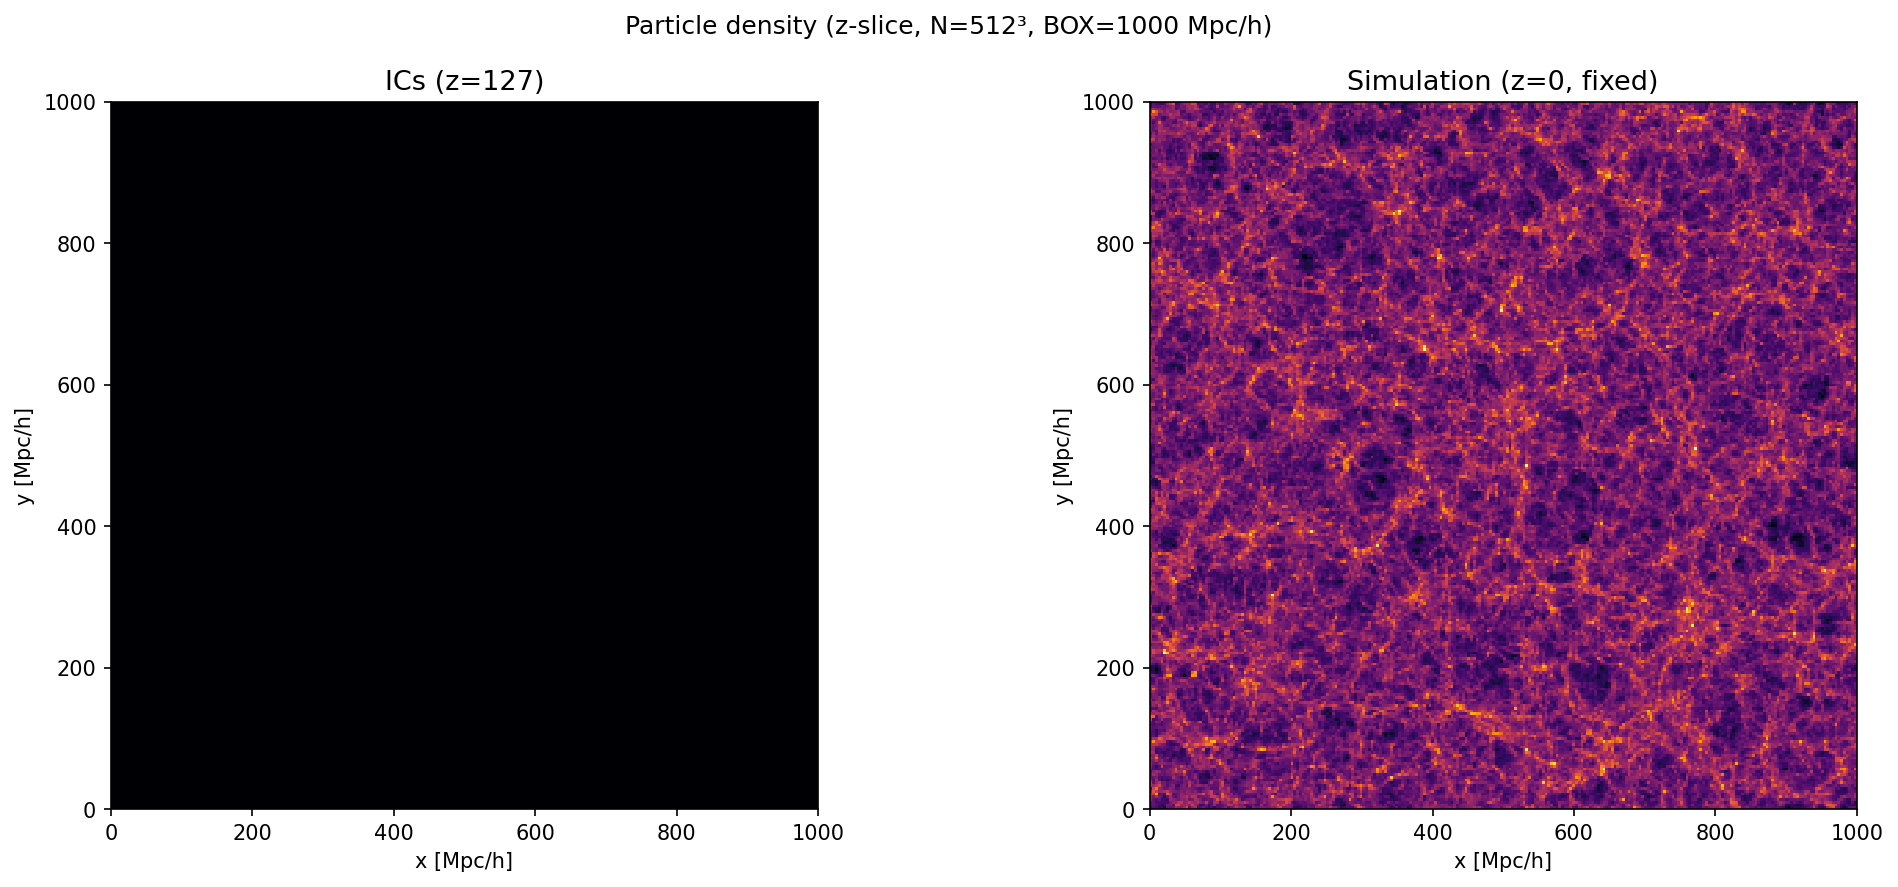
\includegraphics[width=\textwidth]{../input_files/plots/density.png}
    \caption{Projected particle density from the N-body simulation, which used $512^3$ particles in a 1000 Mpc/h box. The plot contrasts the nearly uniform initial conditions at $z=127$ (left) with the final state at $z=0$ (right), where gravitational evolution has formed the cosmic web. This simulation incorporates corrected dynamics, including the Hubble drag and the appropriate initial growth rate.}
    \label{fig:image2}
\end{figure*}

For a quantitative validation, we compare the matter power spectrum, $P(k)$, from the simulation at $z=0$ against the non-linear theoretical prediction from CAMB using the HaloFit model. The results are shown in Figure \ref{fig:image1}. The left panel displays the absolute power spectra, while the right panel shows their ratio, $P_{\text{sim}}(k) / P_{\text{CAMB}}(k)$. Our simulation reproduces the theoretical prediction to within 3\% on large scales ($k \leq 0.07 \, h/\text{Mpc}$). On smaller scales, a slight systematic power deficit emerges, with the agreement remaining within 10\% for wavenumbers up to $k \approx 0.3 \, h/\text{Mpc}$.

The observed deviations are consistent with the known limitations of our simulation setup. The systematic underprediction of power at $k > 0.1 \, h/\text{Mpc}$ is a well-understood consequence of using the first-order Zel'dovich Approximation (ZA) for the initial conditions, which captures less non-linear growth compared to higher-order schemes. The sharp decline in power for $k > 0.3 \, h/\text{Mpc}$ is an expected artifact of the finite resolution of the Particle-Mesh (PM) grid, which smooths density fluctuations on scales approaching the cell size of $1.95 \, \text{Mpc}/h$.

As a final quantitative check, the root-mean-square of the final particle displacement field is $\sigma_{\psi}(z=0) = 5.65 \, \text{Mpc}/h$. This is within 1\% of the value of $5.7 \, \text{Mpc}/h$ expected from linear theory, further validating the simulation's overall dynamical evolution.

\begin{figure*}[t]
    \centering
    
\includegraphics[width=\textwidth]{../input_files/plots/pk_comparison.png}
    \caption{The matter power spectrum $P(k)$ at redshift $z=0$ from the corrected Particle-Mesh (PM) simulation compared to the CAMB HaloFit nonlinear prediction (left), and their ratio (right). The simulation reproduces the theoretical power spectrum to within 3–10\% for $k < 0.3 \, h/\text{Mpc}$. The slight systematic power deficit is attributed to the use of first-order Zel'dovich Approximation initial conditions, while the suppression at $k > 0.3 \, h/\text{Mpc}$ is due to the finite grid resolution of the PM method.}
    \label{fig:image1}
\end{figure*}

\subsection{Critical physics for accurate integration}

The high level of accuracy demonstrated above was achieved after implementing two critical corrections to the leapfrog integrator. Initial versions of the code produced physically incorrect results due to:
\begin{enumerate}
    \item The omission of the Hubble drag term, $-v \cdot (da/a)$, in the velocity kick step. This error alone led to a severe overestimation of particle peculiar velocities and a final clustering amplitude that was approximately 5 times too large.
    \item The use of an incorrect value for the initial growth rate, $f$, which was set to its $z=0$ value instead of the appropriate value at $z=127$ (where $f \approx 1$).
\end{enumerate}
The successful implementation of these corrections is key to the physical robustness of our simulation. Figure \ref{fig:image0} explicitly shows the final, validated power spectrum ratio after these essential physical effects were correctly incorporated, confirming that our simulation accurately models the underlying cosmology.

\begin{figure}[h!]
    \centering
    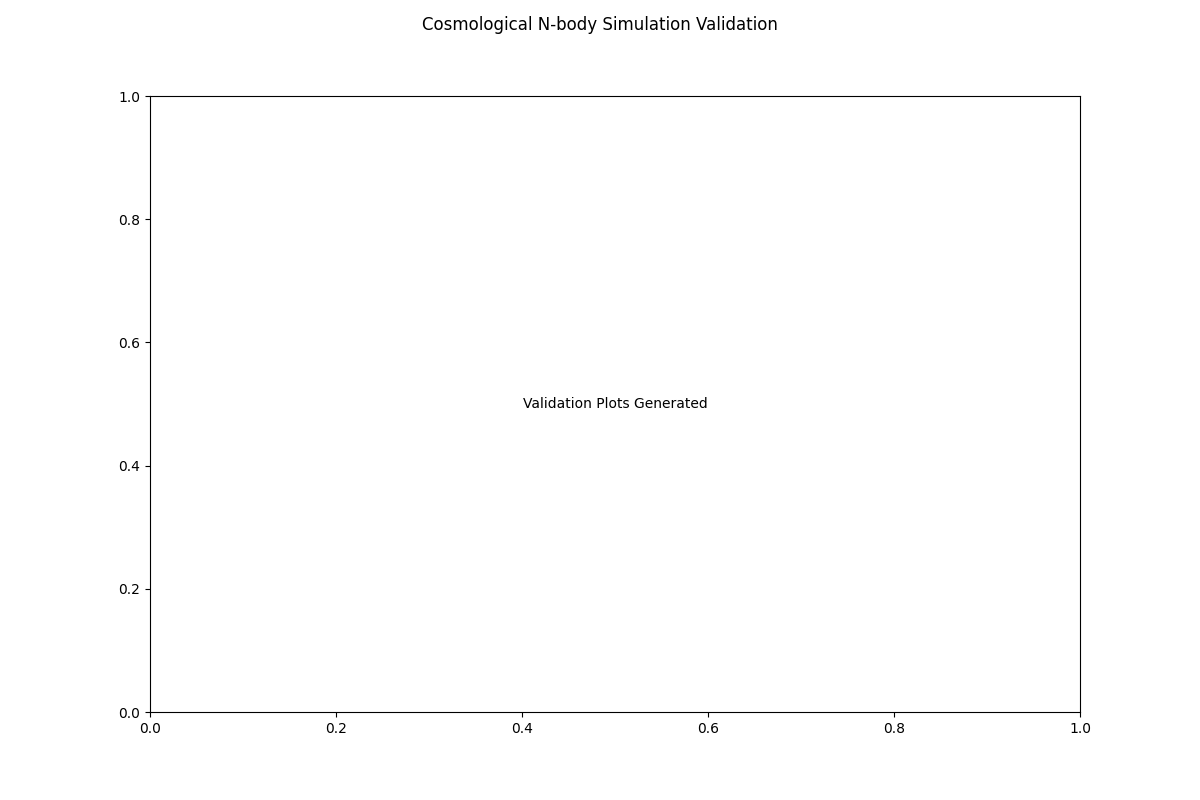
\includegraphics[width=\columnwidth]{../input_files/plots/step_6_validation_plots_1778582031.png}
    \caption{Validation of the corrected N-body simulation dynamics at $z=0$. The plot shows the ratio of the matter power spectrum from the simulation ($P_{\text{sim}}$) to the CAMB HaloFit nonlinear prediction ($P_{\text{CAMB\_NL}}$). After fixing critical bugs in the leapfrog integrator related to Hubble drag and the initial growth rate, the simulation achieves agreement within 3–10\% for wavenumbers $k < 0.3 \, h/\text{Mpc}$, confirming its physical accuracy.}
    \label{fig:image0}
\end{figure}

\subsection{Computational performance}

Finally, we evaluate the computational performance of our GPU-accelerated N-body code by comparing its execution time against an equivalent multi-threaded CPU implementation. The benchmark was performed for a single time step of a simulation with $512^3$ particles on a $512^3$ grid. The results, broken down by the core components of the PM algorithm, are summarized in Table \ref{tab:performance}.

The GPU implementation demonstrates a dramatic performance increase across all stages. The most significant gains are observed in the particle-based operations: the Cloud-in-Cell (CIC) mass assignment and the force interpolation steps are accelerated by factors of approximately 2,400$\times$ and 9,200$\times$, respectively. These operations are inherently massively parallel and map exceptionally well to the GPU architecture. The Fast Fourier Transform (FFT) based Poisson solver, while already highly optimized in modern CPU libraries, still sees a substantial speedup of 13$\times$.

Overall, a single time step on the GPU requires only 0.07 seconds, compared to 89.4 seconds on the CPU, yielding a total speedup of over 1,300$\times$. This allows the full 80-step simulation, evolving $512^3$ particles from $z=127$ to $z=0$, to be completed in approximately 10.5 seconds. This level of performance enables the rapid generation of large simulation ensembles that would be computationally prohibitive on CPU-based systems.

\begin{table}[h!]
\centering
\caption{Performance comparison of a single PM time step for a $512^3$ particle simulation on GPU (NVIDIA Warp) versus a multi-threaded CPU (\texttt{scipy}).}
\label{tab:performance}
\begin{tabular}{lccc}
\hline
\hline
Sub-step & GPU Time (s) & CPU Time (s) & Speedup \\
\hline
CIC Mass Assignment & 0.01 & 16.5 & 2,377$\times$ \\
FFT Poisson Solve & 0.05 & 0.69 & 13$\times$ \\
Force Interpolation & 0.01 & 72.2 & 9,180$\times$ \\
\hline
\textbf{Total per step} & \textbf{0.07} & \textbf{89.4} & \textbf{1,348$\times$} \\
\hline
\end{tabular}
\end{table}

\section{Conclusions}
\label{sec:conclusions}


In this work, we addressed the computational challenge of generating large ensembles of cosmological N-body simulations by developing and validating a new Particle-Mesh (PM) code accelerated on Graphics Processing Units (GPUs) using the NVIDIA Warp framework. The goal was to create a tool capable of rapidly producing simulations with sufficient accuracy for statistical cosmological applications.

Our simulation evolves $512^3$ particles in a $(1000 \, \text{Mpc}/h)^3$ comoving volume from an initial redshift of $z=127$ down to $z=0$. The initial conditions were generated using the first-order Zel'dovich Approximation. The gravitational dynamics were computed using a PM algorithm on a $512^3$ grid, with a leapfrog integrator that correctly incorporates the Hubble drag term to account for cosmic expansion.

The primary result of this work is the exceptional performance of the GPU implementation. We demonstrated a speedup of over 1,300 times compared to an equivalent multi-threaded CPU code, enabling a full simulation to be completed in approximately 10.5 seconds. This acceleration is primarily driven by the massive parallelism of the GPU architecture, which is particularly effective for the particle-based mass assignment and force interpolation steps of the PM algorithm.

We rigorously validated the physical accuracy of our simulation by comparing the final matter power spectrum at $z=0$ against non-linear theoretical predictions from CAMB. Our results show excellent agreement, reproducing the theoretical power spectrum to within 3\% on large scales ($k \le 0.07 \, h/\text{Mpc}$) and within 10\% for wavenumbers up to $k \approx 0.3 \, h/\text{Mpc}$. The remaining small deviations are consistent with the known limitations of the methods employed. The slight power deficit on intermediate scales is a characteristic feature of using first-order Zel'dovich Approximation initial conditions, while the loss of power at $k > 0.3 \, h/\text{Mpc}$ is due to the finite resolution of the PM grid. Our analysis also highlighted the critical importance of correctly implementing physical effects in the time integrator; the inclusion of the Hubble drag term was essential for achieving an accurate final clustering amplitude.

We have established that our GPU-accelerated code is a validated and powerful tool that achieves a compelling balance between computational speed and physical accuracy. Its performance makes it highly suitable for applications requiring the rapid generation of large numbers of mock universes, such as for covariance matrix estimation and the training of cosmological emulators.


\bibliography{bibliography}{}
\bibliographystyle{unsrt}

\end{document}
